\section{Model-free evaluation of policy}

\newcommand{\lr}{\eta}

\begin{frame} 
\mode<presentation>{
    \begin{center} \huge
        \secname
    \end{center}  
    }
    \begin{center}
    \underline{Last time}: Model-based $\corresponds$ offline-planning.\\
    \underline{Today}: Model-free $\corresponds$ inductive online-planning.\\
    \end{center}
\end{frame}

\begin{frame}\frametitle{\secname}

Motivation for model-free evaluation methods:\\

\slidesonly{\vspace{5mm}}

The MDP is not explicitly available, i.e. \notesonly{\textcolor{trans}the transition model }${\color{trans}P}$ and \notesonly{\textcolor{reward}the reward function }${\color{reward}r}$ are unknown and have to be ``experienced''.\\

\slidesonly{\vspace{5mm}}

Options:
\begin{enumerate}[A]
\item Monte-Carlo estimation of $V^\pi(\vec x)$
\item Inductive value estimation through temporal difference learning (TD-Learning)
\end{enumerate}

\end{frame}

\subsection{Monte-Carlo estimation of the value function}

\begin{frame}\frametitle{Model-free option A:~\subsecname}

Monte-Carlo estimation:

	\begin{itemize}
		\item sampling of sequences: step-by-step construction of states, actions and rewards to form possible markov chains
		\item We deal with a finite approximation of infinite Markov chains. This implies:
			\begin{itemize}
				\item rewards weighted by $\gamma^H < \epsilon$ are neglected
				\item value is the discounted reward \textbf{averaged} over $n$ Markov chains of length $H$. \notesonly{This averaging is what leads to the estimates of the state values.}
			\end{itemize}
		
		\question{What are your thoughts about the efficiency of Monte-Carlo estimation?}
		
		\pause 
		
		\item Monte-Carlo estimation requires drawing $n$ chains 
			from the same initial state %$\vec x^{(0)}$
		\item $n$ must be sufficiently large
		\item every state must be evaluated often 
			$\leadsto$ not sample efficient
	\end{itemize}
	
\end{frame}

\subsubsection{Inductive value estimation}

\begin{frame}\frametitle{\subsecname:~\subsubsecname}

	Recall the Bellman equation:
	\begin{equation}
			V^\pi(\vec x_i) \;\;=\;\;
				{\color{policy} \smallsum{k=1}A 
					\pi(\vec a_k \,|\, \vec x_i)}~ 
					{\color{reward} r(\vec x_i, \vec a_k)}
				\;+\; \gamma {\color{trans} \smallsum{j=1}{S}}
					{\color{policy} \smallsum{k=1}A 
					\pi(\vec a_k \,|\, \vec x_i)}~
					{\color{trans} P(\vec x_j \,|\, \vec x_i, \vec a_k)} V^\pi(\vec x_j)
	\end{equation}
		
	\begin{itemize}
		\item But the reward, ${\color{reward} r(\vec x_i, \vec a_k)}$, and the transition model, ${\color{trans}P(\vec  x_j | \vec  x_i, \vec  a_k)}$
		 may not be available to the agent (motivation for model-free evaluation)
		 
		 \pause
		 
		 \slidesonly{\vspace{5mm}}
		 
		\item Inductive value estimation: \underline{Estimating} the value function by sampling from one long Markov chain, i.e.
			\begin{enumerate}
				\item actions are drawn according to the {\color{policy}policy} 
				$ \vec a^{(t)} \sim {\color{policy}\pi(\cdot|\, \vec x^{(t)})}$
				
				\item which lead to {\color{trans}transitions} 
					${\color{trans}\vec x^{(t+1)}
					\sim P(\cdot|\vec x^{(t)},\vec a^{(t)})}$
					
				\item and yield immediate {\color{reward} rewards 
					$r(\vec x^{(t)},\vec a^{(t)})$}
			\end{enumerate}
	\end{itemize}
	
\end{frame}

\mode<presentation>{
\begin{frame}\frametitle{\secname}

Options:
\begin{enumerate}[A]
\item \textcolor{gray}{Monte-Carlo estimation of $V^\pi(\vec x)$}
\item Inductive value estimation through temporal difference learning (TD learning)
\end{enumerate}

\end{frame}
}

\subsection{Temporal difference (TD) learning}

% -----------------------------------------------------------------------------
\begin{frame}\frametitle{Model-free option B:~\subsecname}

%\notesonly{
Temporal difference learning (TD learning) is also a form of inductive value estimation.
%}

\mode<presentation>{
		\begin{enumerate}
			\item actions are drawn according to the {\color{policy}policy} 
		 	$ \vec a^{(t)} \sim {\color{policy}\pi(\cdot|\, \vec x^{(t)})}$
		 	
			\item which lead to {\color{trans}transitions} 
		 		${\color{trans}\vec x^{(t+1)}
		 		\sim P(\cdot|\vec x^{(t)},\vec a^{(t)})}$
		 		
			\item and yield immediate {\color{reward} rewards 
		 		$r(\vec x^{(t)},\vec a^{(t)}) =: r{(t)}$}
		\end{enumerate}
}

\pause 

\vspace{2mm}

TD learning is the asynchronous on-line update of the value function one state at a time
	\slidesonly{\vspace{-8mm}}
	
	\begin{equation}
		\tilde V^{\pi}_{(t+1)}(\vec x^{(t)}) \; = \; 
		\tilde V^{\pi}_{(t)}(\vec x^{(t)}) \;+\;
		\lr \Big( \underbrace{{\color{reward}r^{(t)}} 
		+ \overbrace{
		\gamma \tilde V^{\pi}_{(t)}({\color{trans}\vec x^{(t+1)}})
		}^{\substack{\text{discounted value of}\\ \text{the next step}}} 
		- \tilde V^{\pi}_{(t)}{(\vec x^{(t)})}}_{\text{TD-error }\Delta V_{(t)}} \Big) 
		\label{eq:tdlearningvalue}
	\end{equation}
	
	where $\eta$ is the learning rate\notesonly{, ${\color{reward}r^{(t)}}$ is short for the immediate ${\color{reward}r(\vec x^{(t)},\vec a^{(t)})}$.}
	
	\only<2>{
	Basically,
	\begin{equation}
		\mathit{Esimate_{New}} = \mathit{Esimate_{old}} + \lr \Big(\mathit{Target} - \mathit{Esimate_{old}} \Big)
	\end{equation}
	}
	\only<3>{

	\begin{itemize}
	
	\item  Model knowledge is not required.\notesonly{ We  don't need the complete reward function or the transition model.}
	\notesonly{
	\item \notesonly{TD learning} named after the difference $\Delta V_{(t)}$ in value function estimates (TD-error)
	}
	\end{itemize}
	}
	
\end{frame}

\subsubsection{Relation of Model-free TD learning to model-based value iteration}

\begin{frame}\frametitle{\subsubsecname}

\begin{itemize}
	\item TD learning performs value iteration \emph{on average}
		\vspace{1mm}
		
		\pause
		
		\begin{itemize}
			\item Taking the expectation over all Markov chains 
			that pass~$\vec x_i$~at~time~$t$~reads~$(\vec x^{(t)} = \vec x_i)$ yields:
			
			\begin{equation}
		\underbrace{\E\big\lbrack\tilde V^\pi_{(t+1)}(\vec x^{(t)})\big\rbrack
			}_{\tilde v_i^{\pi(t+1)}}
		\,=\, 
		(1 - \lr)\underbrace{\E\big\lbrack \tilde V^\pi_{(t)}(\vec x^{(t)}) \big\rbrack
			}_{\tilde v_i^{\pi(t)}}
		\,+\, \lr \Big( \underbrace{\E\lbrack{\color{reward} r^{(t)}}\rbrack
		+ \gamma \E\big\lbrack\tilde V^\pi_{(t)}({\color{trans}\vec x^{(t+1)}})\big\rbrack
		}_{({\color{reward} \vec r^\pi} 
			+ \gamma {\color{trans} \vec P^\pi} \tilde{\vec v}^{\pi(t)})_i}\Big)
			\end{equation}
			
		\notesonly{Which we recognize as \emph{value iteration} \slidesonly{from last time}.}
			
		\end{itemize}
	
	
	\vspace{2mm}
	\item TD learning provides an {\em asynchronous online estimate} of 
			$\hat B^\pi[\tilde{\vec v}^{\pi(t)}] = {\color{reward}\vec r^\pi} 
			+ \gamma {\color{trans}\vec P^\pi} \tilde{\vec v}^{\pi(t)}$
		\vspace{1mm}
		\begin{itemize}
%			\setlength{\itemindent}{-1.8em}
			\item asynchronous update of one state at a time
					\vspace{1mm}
			\item model knowledge not required!
		\end{itemize}

	\end{itemize}

\end{frame}

\newpage

\subsubsection{TD learning contracts but does not converge}

\begin{frame}\frametitle{\subsecname}

\notesonly{To contract but to \underline{not} converge means that}\slidesonly{ i.e.} for $t\rightarrow \infty$ and $\eta > 0$ TD learning will \underline{fluctuate} around the true value
and will not stop fluctuating. Holds for ergodic Markov chains

	\begin{block}{Ergodicity}
		A Markov chain is \textbf{ergodic} if it is
		\textbf{positively recurrent} 
		(non-zero probability to leave any state and 
		%a probability of 1 to 
		eventually return to it) and \textbf{aperiodic} 
		(returns to the same state occur at irregular times).
	\end{block}
	
	\slidesonly{
	\vspace{5mm}
	}
	
	%\question{For what transition probabilities would this markov chain become ergodic?}
	
	%\begin{center}
	%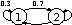
\includegraphics[width=0.4\textwidth]{img/markov_chain_ergodic}
	%\end{center}

\end{frame}

\begin{frame}\frametitle{\subsecname}

Random walk example with stochastic Markov chain with 10 states:
	\begin{itemize}
		\item two randomly initialized 
			value functions ({\color{red}red}/{\color{blue}blue})
		\vspace{1mm}
		 \item deterministic transitions but stochastic policy
		 \vspace{1mm}
		 \item rightmost state is rewarded, $\gamma=0.95$, $\lr=0.5$
		\end{itemize}	

	\begin{center}
		\hspace{-15mm}
		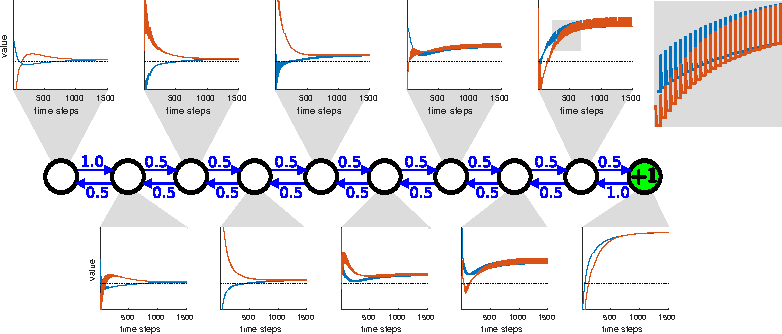
\includegraphics[width=\notesonly{0.9}\slidesonly{0.92}\textwidth]{img/rl_chain_valuecontraction}
		\mode<article>{
		\captionof{figure}{A random walk example in which TD learning will continue fluctuating around the true value but not converge to it.}
		}
	\end{center}

\end{frame}

\subsubsection{Influence of learning rate on TD learning}

\begin{frame}\frametitle{\subsubsecname}

\question{How does the learning rate $\lr$ affect the values obtained through TD learning?}

\mode<presentation>{
	\begin{center}
		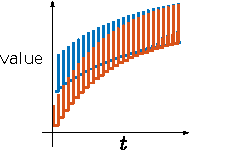
\includegraphics[width=0.3\textwidth]{img/rl_chain_valuecontraction_sub}
	\end{center}
	}
	
\pause

	\begin{itemize}
		\item { large $\eta$: 
			fast learning, large variance (strong fluctuations)}
		\vspace{1mm}
		\item { small $\eta$: 
			slow learning, small variance}
		\vspace{1mm}
		\item { $\eta_{(t)}$ should decay over time, but finding a good annealing schedule may be difficult in practice}
	\end{itemize}

\end{frame}

\subsubsection{Pros \& cons of TD learning}

\begin{frame}\frametitle{\subsubsecname}

\begin{itemize}
\item TD learning learns the value function under policy $\pi$ in an online fashion
\item Every time step updates our guess of the value of one of the states
\end{itemize}

\vspace{10mm}

Pros:
\begin{itemize}
	\item start learning \underline{before} finding out the outcome. We don't have to wait for the reward at the end.
	\item learn online without a final outcome. We can learn from incomplete sequences and non-terminating sequences.
\end{itemize}

Cons:
\pause
\begin{itemize}
	\item biased (we get bad value estimates for states that rarely get sampled and we don't get to choose which state will get sampled next.)
	\item sensitive to the initial state.
\end{itemize}

cf. lecture for more model-free approaches.%: Eligibility Traces \& TD($\lambda$), Batch Value Estimation, ...

\end{frame}

